\title{Computational Genomics: Sequences \\
\large Homework 1
}
\author{
Srinivas Suresh
}
\date{\today}


\documentclass[12pt]{article}

\usepackage{enumitem}

\usepackage{listings}
\usepackage{graphicx}
\usepackage{color}

\definecolor{dkgreen}{rgb}{0,0.6,0}
\definecolor{gray}{rgb}{0.5,0.5,0.5}
\definecolor{mauve}{rgb}{0.58,0,0.82}

\lstset{frame=tb,
language=Python,
aboveskip=3mm,
belowskip=3mm,
showstringspaces=false,
columns=flexible,
basicstyle={\small\ttfamily},
numbers=none,
numberstyle=\tiny\color{gray},
keywordstyle=\color{blue},
commentstyle=\color{dkgreen},
stringstyle=\color{mauve},
breaklines=true,
breakatwhitespace=true,
tabsize=3
}

\begin{document}
\maketitle

\section*{Answers}
Some answers are instructions on how to run the associated program
\begin{enumerate}
    \item answer1.py $>$ inputfile $<$ outputfile
    \begin{enumerate}[label=(\alph*)]
            \item Yes, the sequencer could not determine the 67th nucleotide quite often in every read
            \item
            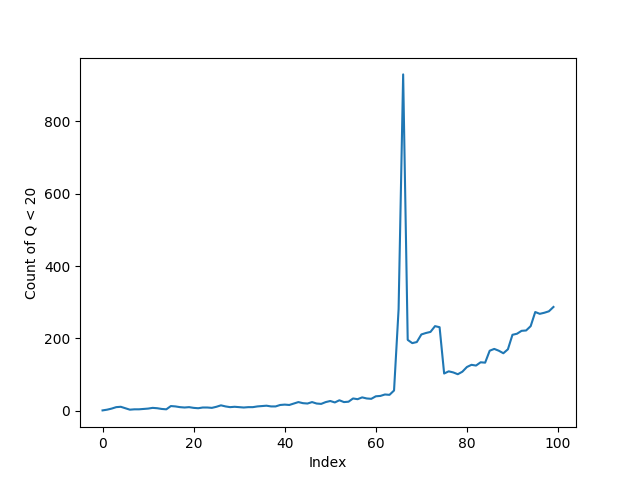
\includegraphics[scale=0.651]{trend.png} 
            \\There appears to be an increase in bases with $Q < 20$ as the index increases. This tells me that the 
            longer the sequence the lower the quality of bases at the end
            
        
    \end{enumerate}
    \item Winner indicated in \textbf{Bold}
    \begin{enumerate}[label=(\alph*)]
        \item 
        Bad Character Rule: 2 moves, 1 skip
         \\ \textbf{Good Suffix Rule: 8 moves, 7 skips}
        \item
        \textbf{Bad Character Rule: 8 moves, 7 skips}
        \\ Good Suffix Rule: 4 moves, 3 skips
        \item
        Bad Character Rule: 5 moves, 4 skip 
        \\ \textbf{Good Suffix Rule: 10 moves, 9 skips}
    \end{enumerate}
    \item Winner indicated in \textbf{Bold}, the answer for case b changes
    \begin{enumerate}[label=(\alph*)]
        \item 
        Bad Character Rule: 2 moves, 1 skip
         \\ \textbf{Good Suffix Rule: 8 moves, 7 skips}
        \item
        \textbf{Bad Character Rule: 8 moves, 7 skips}
        \\ \textbf{Good Suffix Rule: 8 moves, 7 skips}
        \item
        Bad Character Rule: 2 moves, 1 skips 
        \\ \textbf{Good Suffix Rule: 11 moves, 10 skips}
    \end{enumerate}.
    \item Send a pattern in via stdin, ensure complete works file is in same dir is in the same dir To run, call 
    \textit{answer4.py $<$pattern$>$}
\end{enumerate}

\bibliographystyle{abbrv}
\bibliography{main}

\end{document}